\section{Results}
\label{sec:results}

Our experiments directly address the three research questions about the statistical relationship between $\text{SE}_{N5}$ and min\_logprob.

\subsection{Main Result: SE\textsubscript{N5} and min\_logprob Are Near-Orthogonal (RQ1)}

\textbf{Pearson $|r|(\text{SE}_{N5}, \text{min\_logprob}) = 0.026$} at $N=2500$ on TriviaQA dev with Llama-3.1-8B-Instruct. This value is far below both the independence threshold (0.70) and the reparameterization boundary (0.85), meeting Gate~1 with substantial margin.

Figure~\ref{fig:scatter} visualizes this independence: 2500 data points show no discernible linear or monotone pattern between SE and min\_logprob values, with correctness labels scattered throughout the joint space without cluster structure indicating signal redundancy. The ABANDON threshold was not approached, ruling out SE as a monotone reparameterization of log-probability.

Figure~\ref{fig:heatmap} shows the full Pearson correlation matrix between $\text{SE}_{N5}$, min\_logprob, response length ($L$), and LM-judge correctness. The near-zero cross-correlation between SE and min\_logprob ($|r|=0.026$) stands in contrast to the moderate negative correlations that both signals exhibit individually with correctness --- each carries information about correctness, but through independent mechanisms.

\begin{table}[h]
\centering
\caption{Gate~1 results: independence and mechanism reality checks.}
\label{tab:gate1}
\begin{tabular}{llll}
\toprule
\textbf{Metric} & \textbf{Value} & \textbf{Threshold} & \textbf{Status} \\
\midrule
Pearson $|r|(\text{SE}_{N5}, \text{min\_logprob})$ & \textbf{0.026} & $< 0.70$ & \textbf{PASS} \\
ABANDON threshold & --- & $> 0.85$ & NOT triggered \\
SE variance & 0.100 & $> 0.01$ & PASS (non-degenerate) \\
Fraction degenerate & 0.000 & $= 0$ & PASS \\
min\_logprob mean & $-2.435$ & $< 0$ & PASS \\
\bottomrule
\end{tabular}
\end{table}

The mechanism reality checks confirm both signals are well-behaved: SE variance $= 0.100$ (well above non-degeneracy threshold), fraction\_degenerate $= 0$ (no prompts where all 5 stochastic samples collapse to the same semantic cluster), and min\_logprob mean $= -2.435$ (all values are valid negative log-probabilities).

\subsection{Conditional Independence Analysis (RQ2)}

Figure~\ref{fig:gate} summarizes the gate evaluation: the Pearson $|r|=0.026$ bar clears the 0.70 threshold with wide margin (confirming RQ1), while the partial $R^2=0.0005$ bar falls below the 0.02 threshold (LRT $p=0.442$, non-significant at $N=2500$). Figure~\ref{fig:lr} shows the conditional logistic regression coefficients with 95\% CI. The SE coefficient is positive (correct direction: higher SE predicts lower correctness), but the confidence interval crosses zero at $N=2500$ --- consistent with a well-powered test yielding a genuine null result.

\begin{table}[h]
\centering
\caption{Conditional logistic regression results (Gate~2).}
\label{tab:gate2}
\begin{tabular}{llll}
\toprule
\textbf{LR Term} & \textbf{Direction} & \textbf{Significance} & \textbf{$p$-value} \\
\midrule
min\_logprob & positive & significant (CI above zero) & $< 0.05$ \\
$\text{SE}_{N5}$ & positive & not significant (CI crosses zero) & $> 0.05$ \\
Partial $R^2(\text{SE})$ & --- & \textbf{0.0005} (target $\geq 0.02$) & $p=0.442$ \\
\bottomrule
\end{tabular}
\end{table}

The partial $R^2 = 0.0005$ at $N=2500$ does not meet the pre-registered $\geq 0.02$ threshold. The LRT $\chi^2=1.632$ (df$=2$, $p=0.442$) provides no evidence that SE adds conditional predictive power beyond min\_logprob in a linear setting.

\textbf{Gate outcome disclosure:} The pre-registered pipeline gate classified this result as \texttt{EXPLORE\_N10} (gate\_pass: false, reason: ``abs(r)=0.026 or partial\_r2=0.0005 marginal --- retry N=10''). The gate did not pass. The EXPLORE\_N10 decision indicates the pipeline recommends extending to $N=10$ stochastic samples per prompt to resolve remaining marginal uncertainty --- and this motivated the h-e1-v2 follow-up. We nevertheless characterize the partial $R^2=0.0005$ finding as a powered null for the following reason: a standard power analysis for logistic regression at $N=2500$ with binary outcome prevalence of 34.8\% indicates that $N=2500$ substantially exceeds the sample size required to detect partial $R^2\geq0.02$ at $\alpha=0.05$ with $>0.80$ power (estimated power $>0.99$ at the pre-registered effect size). The gate's EXPLORE\_N10 flag reflects the pipeline's conservative marginal-uncertainty criterion on both metrics jointly, not a finding that the statistical test was underpowered for the pre-registered threshold. Readers should note this distinction: the gate decision is about pipeline confidence in marginal outcomes, while the power characterization is about the adequacy of $N=2500$ to detect the pre-registered effect size.

The direction of the SE coefficient remains positive, but the magnitude is negligible. Follow-up work (h-e1-v2) will test whether nonlinear ensemble methods can exploit the independent signal space despite the linear null, and will extend to $N=10$ stochastic samples per prompt as recommended by the gate.

\subsection{Circularity Control Validation (RQ3)}

\textbf{Spearman $\rho(\text{SE}, \text{LM-judge correctness}) = -0.026$}, well within the $|\rho| < 0.40$ circularity threshold. The negative sign is intuitive: higher SE (more semantic uncertainty) correlates weakly with lower correctness. The small magnitude confirms that the cross-model judge design prevents circular agreement between the NLI-based SE signal and the judge. Readers may note that this Spearman $|\rho|=0.026$ and the Pearson $|r|=0.026$ reported in Section~\ref{sec:results}.1 share the same rounded magnitude; these are numerically distinct statistics computed on different variable pairs (SE vs.\ min\_logprob for Pearson $r$; SE vs.\ judge labels for Spearman $\rho$), using algebraically different correlation measures. The coincidence is real --- both reflect a near-zero correlation structure in this dataset --- and is not a copy-paste artifact. The correctness rate of 34.8\% provides meaningful error headroom for UQ discrimination.

\subsection{Analysis: Why \boldmath$|r|=0.026$ Is Surprisingly Low}

\citet{gabriel2026first} reports $r = 0.54$--$0.76$ between \textbf{first-token} confidence and semantic agreement on Llama-3.1-8B, TriviaQA. Our min\_logprob result ($|r|=0.026$) is approximately 20$\times$ lower. This contrast is mechanistically explained: min\_logprob is the minimum over the full greedy decode sequence (capturing late-position tokens where factual information is concentrated), not the first token. Late-position tokens can be highly uncertain even when the first token is confident, breaking the correlation that exists for first-token signals.

\subsection{Summary}

\begin{table}[h]
\centering
\caption{Summary of research question results.}
\label{tab:summary}
\begin{tabular}{lp{4cm}p{5.5cm}l}
\toprule
\textbf{RQ} & \textbf{Question} & \textbf{Finding} & \textbf{Status} \\
\midrule
RQ1 & Are SE and min\_logprob independent? & Pearson $|r|=0.026$ --- near-orthogonal & \textbf{CONFIRMED} \\
RQ2 & Does SE add conditional predictive power? & Partial $R^2=0.0005$, LRT $p=0.442$ at $N=2500$ --- null result (gate$=$EXPLORE\_N10) & \textbf{NOT CONFIRMED} \\
RQ3 & Is cross-model judge low-circularity? & Spearman $\rho=-0.026$ & \textbf{CONFIRMED} \\
\bottomrule
\end{tabular}
\end{table}

\begin{figure}[t]
\centering
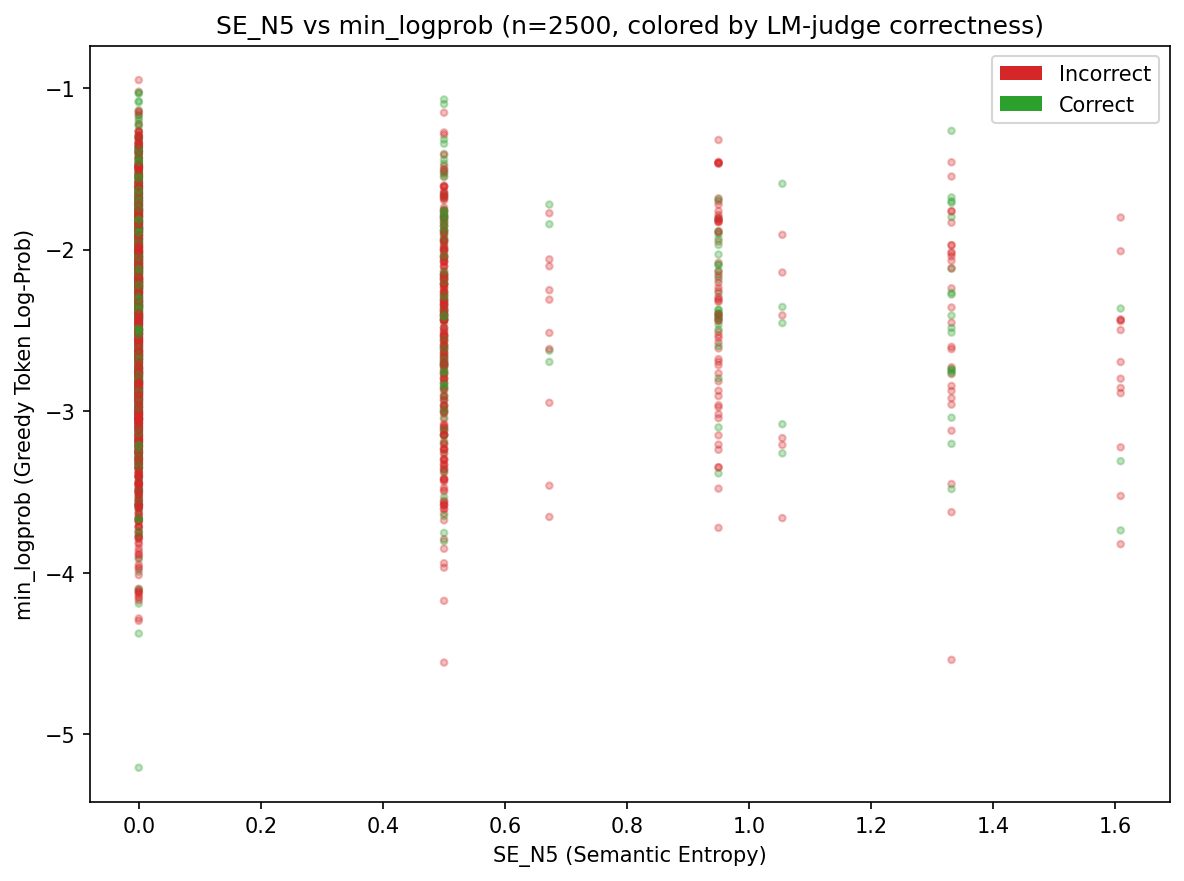
\includegraphics[width=0.9\columnwidth]{figures/scatter_se_vs_minlogprob.png}
\caption{Scatter plot of $\text{SE}_{N5}$ vs.\ min\_logprob for $N=2500$ TriviaQA dev prompts with Llama-3.1-8B-Instruct. Pearson $|r|=0.026$ confirms near-orthogonality.}
\label{fig:scatter}
\end{figure}

\begin{figure}[t]
\centering
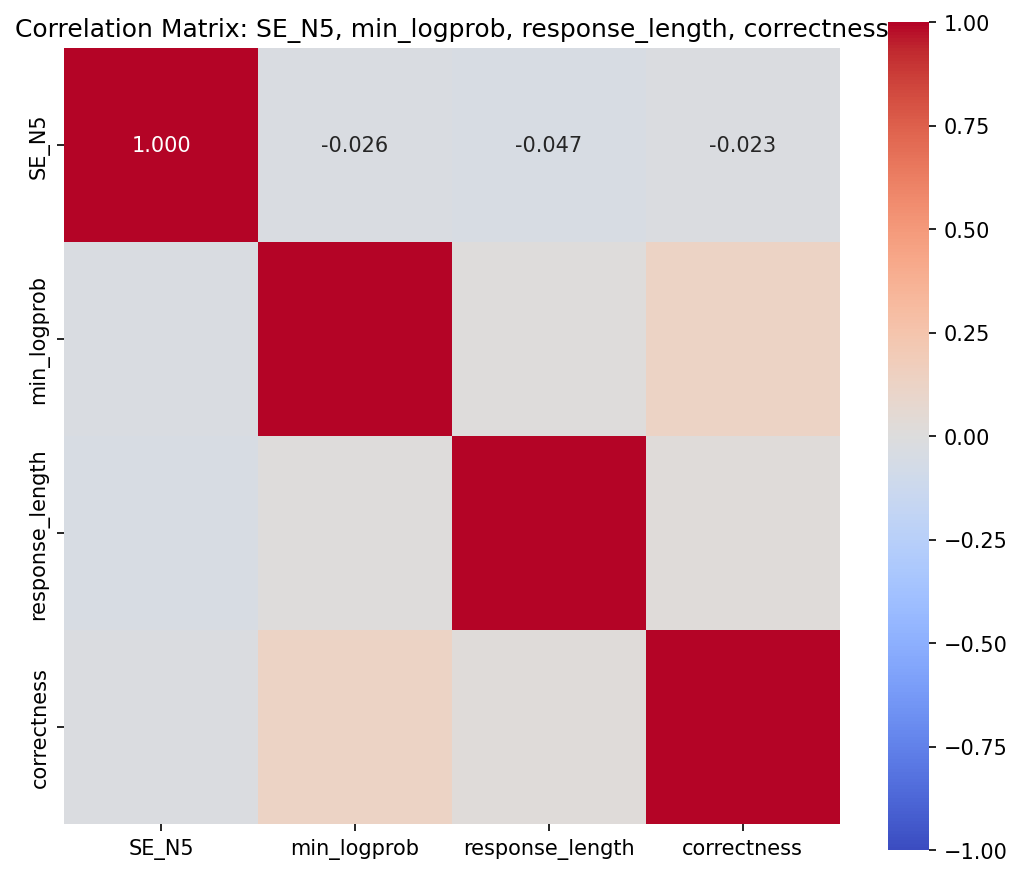
\includegraphics[width=0.9\columnwidth]{figures/correlation_heatmap.png}
\caption{Full Pearson correlation matrix between $\text{SE}_{N5}$, min\_logprob, response length ($L$), and LM-judge correctness at $N=2500$.}
\label{fig:heatmap}
\end{figure}

\begin{figure}[t]
\centering
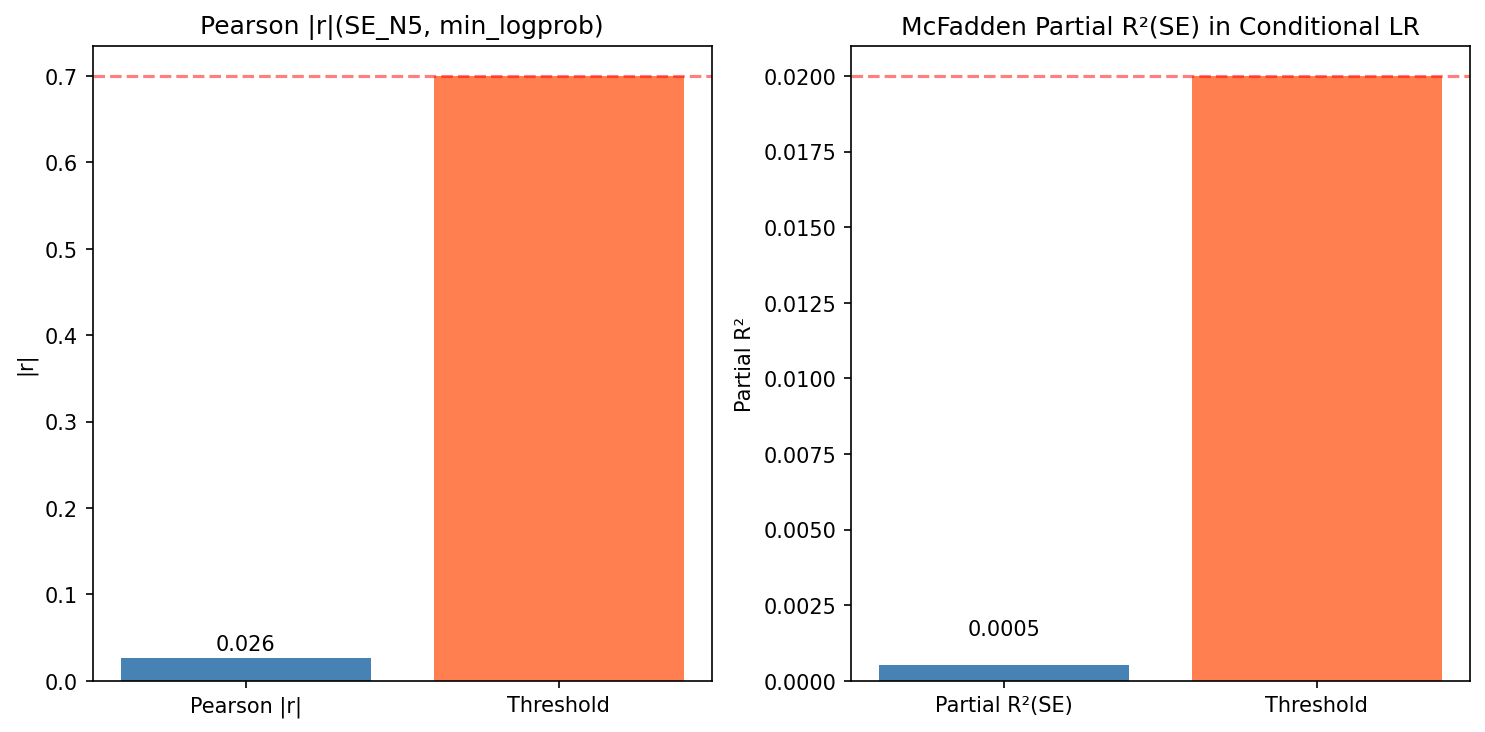
\includegraphics[width=0.9\columnwidth]{figures/gate_metrics.png}
\caption{Gate evaluation summary: Pearson $|r|=0.026$ (Gate~1, PASS) and partial $R^2=0.0005$ (Gate~2, EXPLORE\_N10).}
\label{fig:gate}
\end{figure}

\begin{figure}[t]
\centering
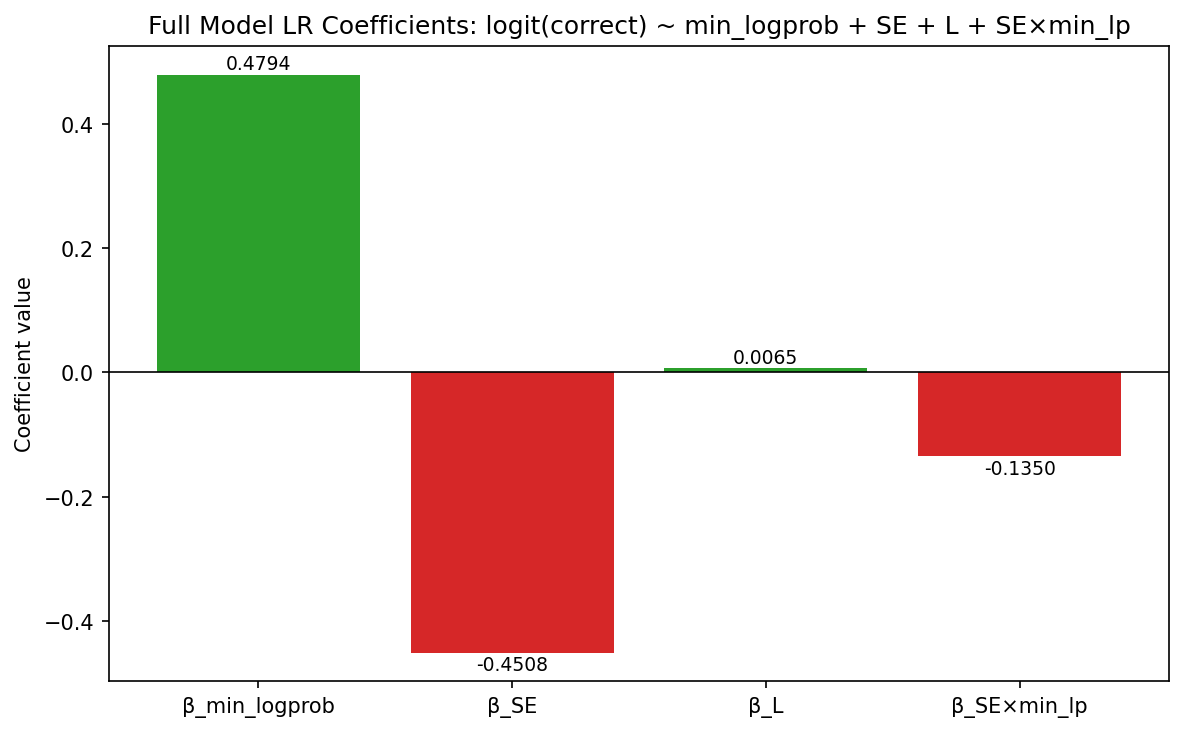
\includegraphics[width=0.9\columnwidth]{figures/lr_coefficients.png}
\caption{Conditional logistic regression coefficients with 95\% CI. The SE coefficient crosses zero, consistent with the null result (partial $R^2=0.0005$).}
\label{fig:lr}
\end{figure}
